\section{Specifikation og Analyse} \label{section:specanal}

I følgende afsnit vil der være beskrevet de overvejelser der har været i forbindelse med den overordnede systemarkitektur.

\begin{figure}[H]
	\centering
	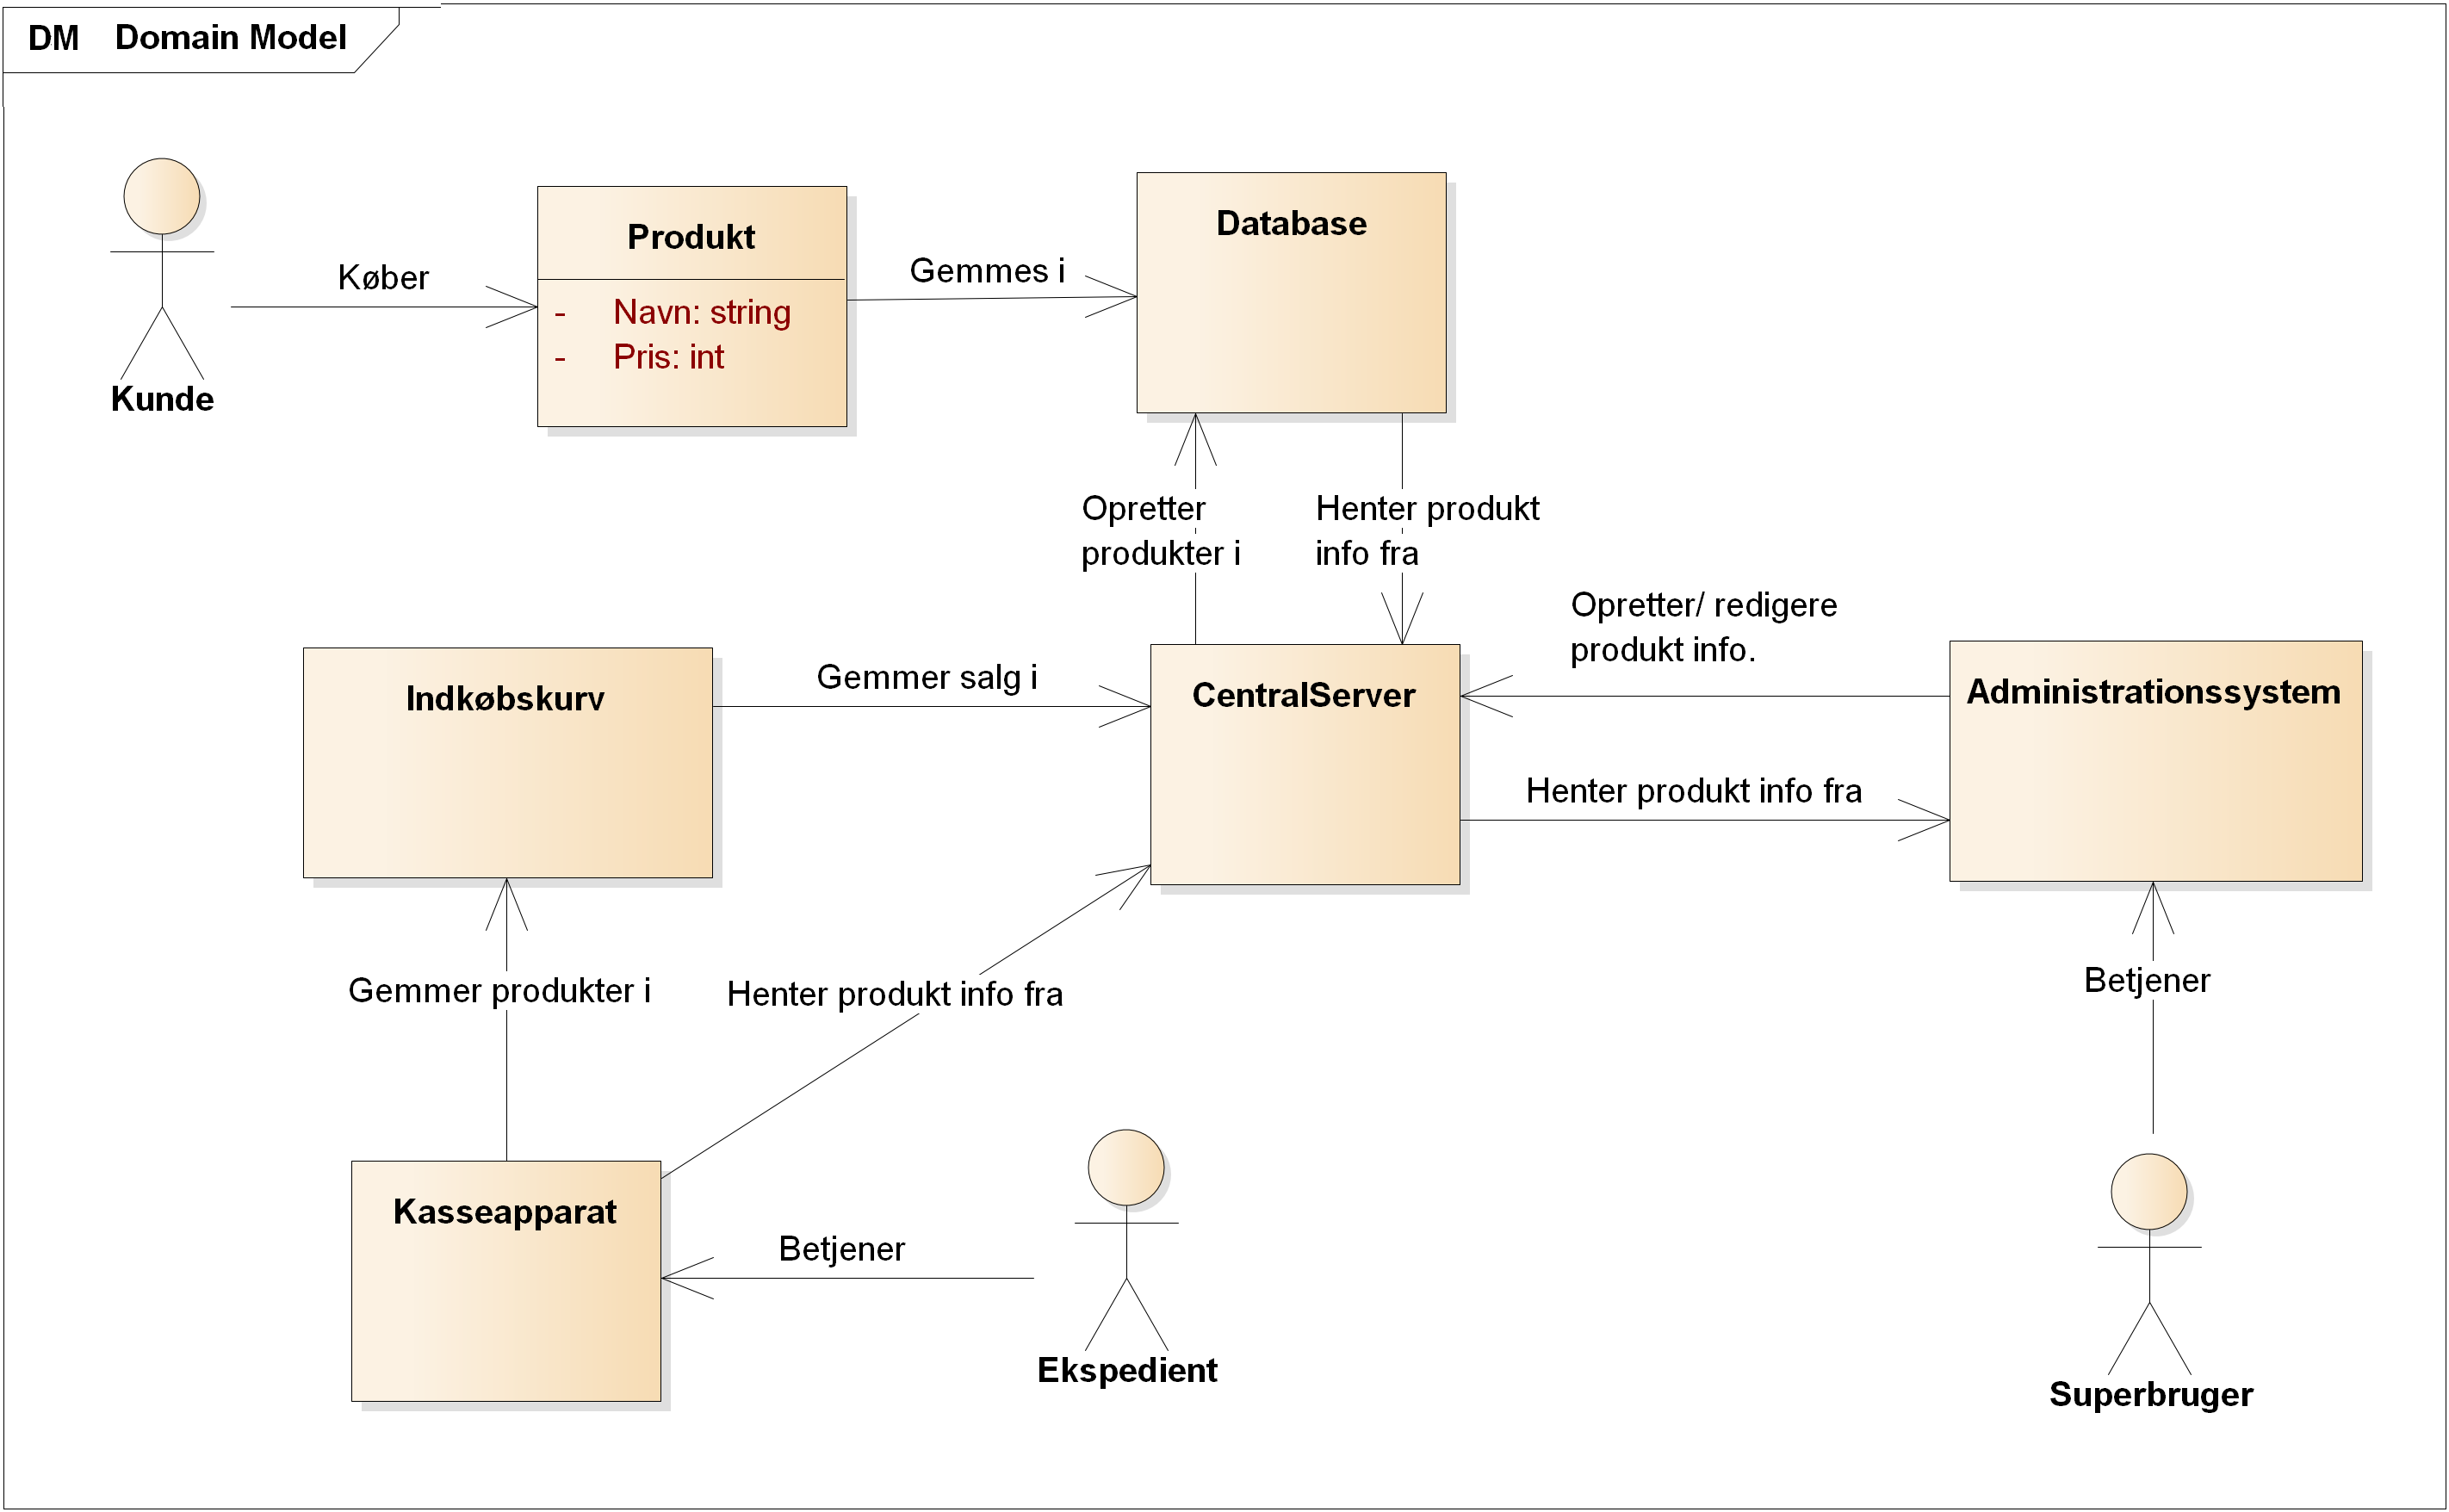
\includegraphics[width=1\textwidth]{Projektbeskrivelse/Images/DomainModel.png}
	\caption{Domænemodel for salgssystemet}
	\label{fig:domain}
\end{figure}


\textbf{Adskillelse af Administrationssystem og Kasseapparat}\\
De to delsystemer tilgås af forskellige aktører til forskellige formål. Det er derfor besluttet, at implementere de to systemer som to forskellige eksekverbare programmer. Dette simplificerer desuden også brugergrænsefladerne i begge systemer.\\

\textbf{Distribuerede systemer}\\
Ift. gruppens overvejelser er det besluttet, at systemet skal understøtte, at både flere kasseapparater og administrationssystemer kan være tilgængelige på samme tid. Det har i den forbindelse været nødvendigt at implementere en central server, hvor en eller flere klienter kan forbinde til, samt kommunikere med, på samme tid. Denne server skal stå for at opbevare persistent data.\\

Denne måde at implementere systemet på har den fordel, at butikskæder med flere butikker kan vedligeholde produktkataloget ét sted, og hurtigt få det distribueret til samtlige butikker.\\

For at imødekomme ovenstående har det været nødvendigt at benytte en kommunikationsvej, der tillader kommunikation over afstand. Læs mere nedenfor under afsnittet "Kommunikation."\\

\textbf{Kommunikation}\\
Til at kommunikkere med CentralServer og klienter\footnote{Eksempelvis Administrationssystem og/eller Kasseapparat}, blev det besluttet at benytte TCP/IP~\cite{TCPIP} som kommunikationsvej.\\

Dette giver følgende fordele:

\begin{itemize}
	\item Der er garanteret fejlfri dataoverførsel.
	\item Fuld duplex kommunikation.
	\item Serveren kan stå hvor som helst i verdenen, så længe den er forbundet til internettet.
	\item TCP/IP er generelt nemt at udvikle til, og er desuden bredt understøttet.
	\item Selvom både TCP- og IP-protokollerne har overhead (metadata) overføres så lidt data mellem delsystemerne, at dette ikke bliver noget problem.
\end{itemize}

\textbf{Kommunikationsprotokol}\\
For at kunne udveksle data mellem CentralServer og Administrationssystem/Kasseapparat, var det nødvendigt at implementere en protokol, som alle tre systemer kunne arbejde med.\\

Det blev i den forbindelse besluttet, at implementere et fælles protokol-lag, som kunne håndtere de lavpraktiske detaljer omkring, hvilket data, der kommunikeres mellem systemerne.\\

Dette har været det oprindelige grundlag for, at indføre et fælles kodebibliotek til de tre delsystemer\footnote{SharedLib}.\\

\textbf{Database og persistent data}\\
Da mange klienter skal kunne tilgå systemets persistente data på samme tid har det været nødvendigt at vælge en model, hvor der ikke kan opstå f.eks. deadlocks eller andre problemer ifm. tilgang til data.\\

Det blev besluttet, at den bedste løsning var at lade CentralServer håndtere alt persistent data. Administrationssystem og Kasseapparat forbinder derfor kun til Database indirekte gennem CentralServer. Det er så CentralCervers ansvar at sørge for, at førnævnte problemer ikke opstår.\\

\textbf{Datamodeller}\\
Datamodellerne vil være delt på tværs af alle tre delsystemer. Ved at definere dem ét sted kan de nemt genbruges. Det blev derfor besluttet, at alle datamodeller skulle implementeres i et fælles kodebibliotek.\\

Det har den naturlige konsekvens, at alle delsystemer skal opdateres, hvis en datamodel bliver opdateret. Dette anses dog ikke for at være et problem.\\